\section{Dínamica general de las cotizaciones}
%Comportamiento de los cotizantes (tdos los dependientes)
%Comportamiento de algunas novedades  (variaciones anuales y mensuales) 2021, 2020 y 2019. Lo mismo retiros. Bajan los ingresos. 
%Contraste con IEM */

%% cuerpo del documento mencionar variaciones anuales. Hablar de variaciones de solo un salario mínimo. 

% Variaciones mensuales con el total.
FABIO 
Tres hojas!  Capitulo 1 
1 - General con contraste ano tipo
2- Cotizantes por rango salarial
3 - Novedaes


\lipsum[2-3] %%%

\begin{table}[!h]
\centering
\begin{minipage}{0.5\textwidth}
  \centering
  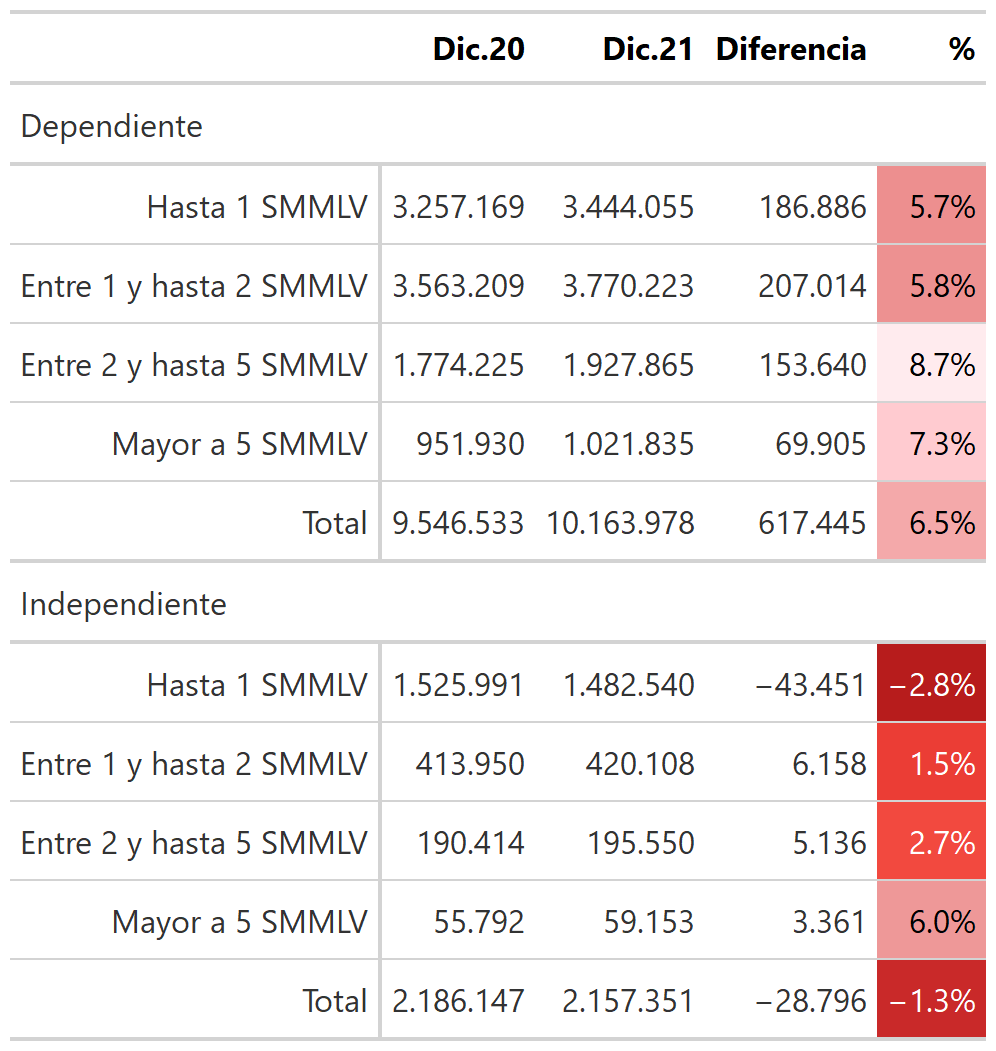
\includegraphics[width=0.6\linewidth]{results/Resumen/salida_table3_total.png}
\end{minipage}%
\begin{minipage}{0.5\textwidth}
  \centering
  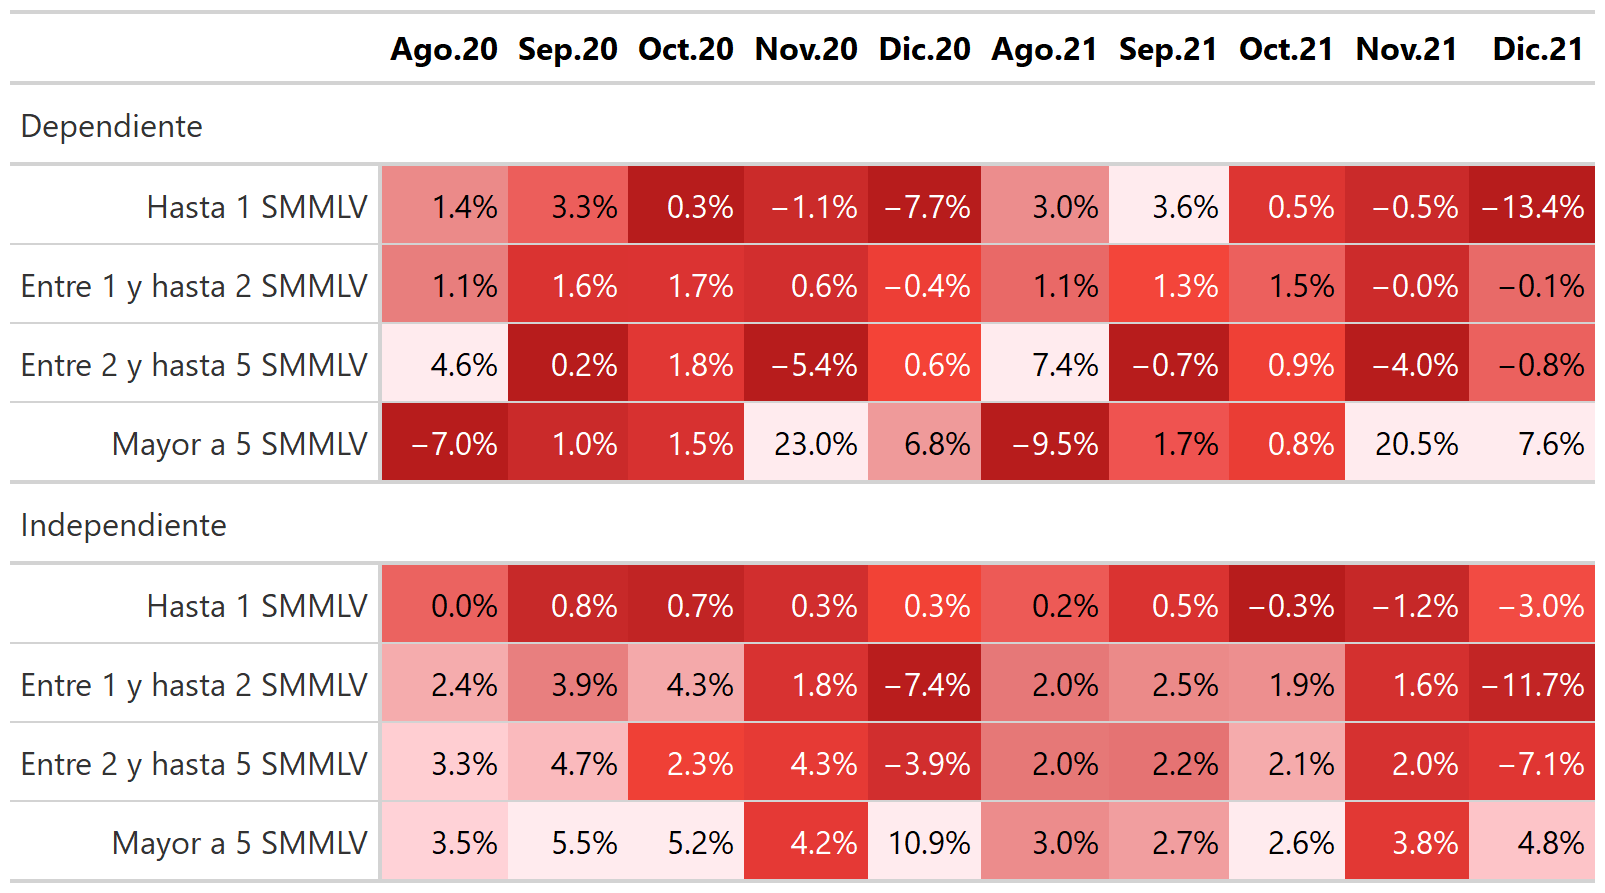
\includegraphics[width=\linewidth]{results/Resumen/salida_table3_variaciones.png}
\end{minipage}
\caption{Resumen número de cotizantes por rango salarial (IBC)}. Totales (Izq.), variaciones mensuales (Der.)
\label{tabla:tabla3}
\end{table}
\lipsum[2-3] %%%
